\begin{frame}
    \frametitle{Natural Language Understanding (NLU)}
    \textbf{My definition:}\\
    NLU means translating natural language into a formal semantic representation.

    \vspace{2em}
    \makebox[9cm]{\str{How many people live in Slovakia?}} $\leadsto\;\;$ \str{5.458 million}

    \vspace{1em}
    \makebox[9cm]{\str{Do more people live in Slovakia than in Thailand?}} $\leadsto\;\;$ ???

    \vspace{2em}
    \centering
    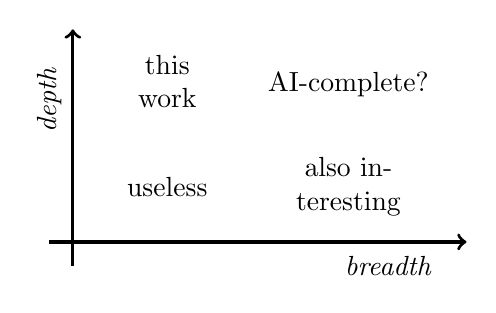
\begin{tikzpicture}
        \node (nbnd) at (1.2,0.7) {useless};
        \node (bnd) at (3.5,0.7) {\begin{tabular}{c}also in-\\teresting\end{tabular}};
        \node (bd) at (3.5,2.0) {AI-complete?};
        \node (nbd) at (1.2,2.0) {\begin{tabular}{c}this\\work\end{tabular}};
        \draw[->,very thick] (-0.3,0) -- (5,0);
        \draw[->,very thick] (0,-0.3) -- (0,2.7);
        \node at (4.0, -0.3) {\itshape breadth};
        \node[rotate=90] at (-0.3,1.8) {\itshape depth};
    \end{tikzpicture}
\end{frame}
